%% The first command in your LaTeX source must be the \documentclass command.
\documentclass[acmtog]{acmart}
\usepackage[english,ngerman]{babel}
\usepackage[utf8]{inputenc}

%% \BibTeX command to typeset BibTeX logo in the docs
\AtBeginDocument{%
  \providecommand\BibTeX{{%
    \normalfont B\kern-0.5em{\scshape i\kern-0.25em b}\kern-0.8em\TeX}}}

\copyrightyear{2024}
\acmYear{2024}
\citestyle{acmauthoryear}

\usepackage[figurename=Fig.]{caption}
\setcopyright{none}
\makeatletter
\renewcommand{\fnum@figure}{Abb. \thefigure}
\makeatother
\addto\captionsngerman{\renewcommand{\figurename}{Abb.}}
\settopmatter{printacmref=false} % Removes citation information below abstract
\renewcommand\footnotetextcopyrightpermission[1]{} % removes footnote with conference information in first column

%%
%% end of the preamble, start of the body of the document source.
\begin{document}

%%
%% The "title" command has an optional parameter,
%% allowing the author to define a "short title" to be used in page headers.
\title{The Name of the Title is Hope}

%%
%% The "author" command and its associated commands are used to define
%% the authors and their affiliations.
%% Of note is the shared affiliation of the first two authors, and the
%% "authornote" and "authornotemark" commands
%% used to denote shared contribution to the research.
\author{A-Vorname A-Nachname}
\authornote{Alle Studierenden trugen zu gleichen Teilen zu dieser Arbeit bei.}
\author{B-Vorname B-Nachname}
\authornotemark[1]
\author{C-Vorname C-Nachname}
\authornotemark[1]
\affiliation{%
	\institution{Hochschule für Technik, Wirtschaft und Kultur Leipzig (HTWK Leipzig)}
	\streetaddress{Karl-Liebknecht-Str. 132}
	\city{Leipzig}
	%\state{Ohio}
	\country{Deutschland}
	\postcode{04277}
}
%%
%% By default, the full list of authors will be used in the page
%% headers. Often, this list is too long, and will overlap
%% other information printed in the page headers. This command allows
%% the author to define a more concise list
%% of authors' names for this purpose.
\renewcommand{\shortauthors}{A-Nachname, B-Nachname und C-Nachname}

%%
%% The abstract is a short summary of the work to be presented in the
%% article.
\begin{abstract}
	(Abstract-Länge ist typischerweise 15-25 Zeilen lang, in der PDF-Darstellung)

	A clear and well-documented \LaTeX\ document is presented as an
	article formatted for publication by ACM in a conference proceedings
	or journal publication. Based on the ``acmart'' document class, this
	article presents and explains many of the common variations, as well
	as many of the formatting elements an author may use in the
	preparation of the documentation of their work.
\end{abstract}

\maketitle

\section{Einleitung und Motivation}

 (Beschreibung von Kontext, Problemen, Anforderungen und Zielen)

ACM's consolidated article template, introduced in 2017, provides a
consistent \LaTeX\ style for use across ACM publications, and
incorporates accessibility and metadata-extraction functionality
necessary for future Digital Library endeavors. Numerous ACM and
SIG-specific \LaTeX\ templates have been examined, and their unique
features incorporated into this single new template.

If you are new to publishing with ACM, this document is a valuable
guide to the process of preparing your work for publication. If you
have published with ACM before, this document provides insight and
instruction into more recent changes to the article template.

The ``\verb|acmart|'' document class can be used to prepare articles
for any ACM publication --- conference or journal, and for any stage
of publication, from review to final ``camera-ready'' copy, to the
author's own version, with {\itshape very} few changes to the source.

(kurze Zusammenfassung der Struktur der Belegarbeit)

Diese Arbeit ist folgendermaßen strukturiert.
In Kapitel ...
...
...
Abschließend ...

\section{Grundlagen}

 (Begriffe und Definitionen)

As noted in the introduction, the ``\verb|acmart|'' document class can
be used to prepare many different kinds of documentation --- a
dual-anonymous initial submission of a full-length technical paper, a
two-page SIGGRAPH Emerging Technologies abstract, a ``camera-ready''
journal article, a SIGCHI Extended Abstract, and more --- all by
selecting the appropriate {\itshape template style} and {\itshape
		template parameters}.

This document will explain the major features of the document
class. For further information, the {\itshape \LaTeX\ User's Guide} is
available from
\url{https://www.acm.org/publications/proceedings-template}.

\subsection{Template Styles}

The primary parameter given to the ``\verb|acmart|'' document class is
the {\itshape template style} which corresponds to the kind of publication
or SIG publishing the work. This parameter is enclosed in square
brackets and is a part of the {\verb|documentclass|} command:
\begin{verbatim}
  \documentclass[STYLE]{acmart}
\end{verbatim}

Journals use one of three template styles. All but three ACM journals
use the {\verb|acmsmall|} template style:
\begin{itemize}
	\item {\verb|acmsmall|}: The default journal template style.
	\item {\verb|acmlarge|}: Used by JOCCH and TAP.
	\item {\verb|acmtog|}: Used by TOG.
\end{itemize}

The majority of conference proceedings documentation will use the {\verb|acmconf|} template style.
\begin{itemize}
	\item {\verb|acmconf|}: The default proceedings template style.
	      \item{\verb|sigchi|}: Used for SIGCHI conference articles.
	      \item{\verb|sigchi-a|}: Used for SIGCHI ``Extended Abstract'' articles.
	      \item{\verb|sigplan|}: Used for SIGPLAN conference articles.
\end{itemize}

\subsection{Template Parameters}

In addition to specifying the {\itshape template style} to be used in
formatting your work, there are a number of {\itshape template parameters}
which modify some part of the applied template style. A complete list
of these parameters can be found in the {\itshape \LaTeX\ User's Guide.}

Frequently-used parameters, or combinations of parameters, include:
\begin{itemize}
	\item {\verb|anonymous,review|}: Suitable for a ``dual-anonymous''
	      conference submission. Anonymizes the work and includes line
	      numbers. Use with the \verb|\acmSubmissionID| command to print the
	      submission's unique ID on each page of the work.
	      \item{\verb|authorversion|}: Produces a version of the work suitable
	      for posting by the author.
	      \item{\verb|screen|}: Produces colored hyperlinks.
\end{itemize}

This document uses the following string as the first command in the
source file:
\begin{verbatim}
\documentclass[acmtog]{acmart}
\end{verbatim}

\section{(Hauptteil mit ggf. mehreren Sections)}

 (der Hauptteil umfasst typischerweise ca. 2/3 bis 3/4 des Texts der Arbeit.)

Modifying the template --- including but not limited to: adjusting
margins, typeface sizes, line spacing, paragraph and list definitions,
and the use of the \verb|\vspace| command to manually adjust the
vertical spacing between elements of your work --- is not allowed.

	{\bfseries Your document will be returned to you for revision if
		modifications are discovered.}

The ``\verb|acmart|'' document class requires the use of the
``Libertine'' typeface family. Your \TeX\ installation should include
this set of packages. Please do not substitute other typefaces. The
``\verb|lmodern|'' and ``\verb|ltimes|'' packages should not be used,
as they will override the built-in typeface families.

The ``\verb|acmart|'' document class includes the ``\verb|booktabs|''
package --- \url{https://ctan.org/pkg/booktabs} --- for preparing
high-quality tables.

Table captions are placed {\itshape above} the table.

Because tables cannot be split across pages, the best placement for
them is typically the top of the page nearest their initial cite.  To
ensure this proper ``floating'' placement of tables, use the
environment \textbf{table} to enclose the table's contents and the
table caption.  The contents of the table itself must go in the
\textbf{tabular} environment, to be aligned properly in rows and
columns, with the desired horizontal and vertical rules.  Again,
detailed instructions on \textbf{tabular} material are found in the
\textit{\LaTeX\ User's Guide}.

Immediately following this sentence is the point at which
Table~\ref{tab:freq} is included in the input file; compare the
placement of the table here with the table in the printed output of
this document.

\begin{table}
	\caption{Frequency of Special Characters}
	\label{tab:freq}
	\begin{tabular}{ccl}
		\toprule
		Non-English or Math & Frequency   & Comments          \\
		\midrule
		\O                  & 1 in 1,000  & For Swedish names \\
		$\pi$               & 1 in 5      & Common in math    \\
		\$                  & 4 in 5      & Used in business  \\
		$\Psi^2_1$          & 1 in 40,000 & Unexplained usage \\
		\bottomrule
	\end{tabular}
\end{table}

To set a wider table, which takes up the whole width of the page's
live area, use the environment \textbf{table*} to enclose the table's
contents and the table caption.  As with a single-column table, this
wide table will ``float'' to a location deemed more
desirable. Immediately following this sentence is the point at which
Table~\ref{tab:commands} is included in the input file; again, it is
instructive to compare the placement of the table here with the table
in the printed output of this document.

\begin{table*}
	\caption{Some Typical Commands (table with full page width)}
	\label{tab:commands}
	\begin{tabular}{ccl}
		\toprule
		Command                    & A Number & Comments         \\
		\midrule
		\texttt{{\char'134}author} & 100      & Author           \\
		\texttt{{\char'134}table}  & 300      & For tables       \\
		\texttt{{\char'134}table*} & 400      & For wider tables \\
		\bottomrule
	\end{tabular}
\end{table*}

Always use midrule to separate table header rows from data rows, and
use it only for this purpose. This enables assistive technologies to
recognise table headers and support their users in navigating tables
more easily.

\subsection{Math Equations}
You may want to display math equations in three distinct styles:
inline, numbered or non-numbered display.  Each of the three are
discussed in the next sections.

\subsubsection{Inline (In-text) Equations}
A formula that appears in the running text is called an inline or
in-text formula.  It is produced by the \textbf{math} environment,
which can be invoked with the usual
\texttt{{\char'134}begin\,\ldots{\char'134}end} construction or with
the short form \texttt{\$\,\ldots\$}. You can use any of the symbols
and structures, from $\alpha$ to $\omega$, available in
\LaTeX~\cite{Lamport:LaTeX}; this section will simply show a few
examples of in-text equations in context. Notice how this equation:
\begin{math}
	\lim_{n\rightarrow \infty}x=0
\end{math},
set here in in-line math style, looks slightly different when
set in display style.  (See next section).

\subsubsection{Display Equations}
A numbered display equation---one set off by vertical space from the
text and centered horizontally---is produced by the \textbf{equation}
environment. An unnumbered display equation is produced by the
\textbf{displaymath} environment.

Again, in either environment, you can use any of the symbols and
structures available in \LaTeX\@; this section will just give a couple
of examples of display equations in context.  First, consider the
equation, shown as an inline equation above:
\begin{equation}
	\lim_{n\rightarrow \infty}x=0
\end{equation}
Notice how it is formatted somewhat differently in
the \textbf{displaymath}
environment.  Now, we'll enter an unnumbered equation:
\begin{displaymath}
	\sum_{i=0}^{\infty} x + 1
\end{displaymath}
and follow it with another numbered equation:
\begin{equation}
	\sum_{i=0}^{\infty}x_i=\int_{0}^{\pi+2} f
\end{equation}
just to demonstrate \LaTeX's able handling of numbering.

The ``\verb|figure|'' environment should be used for figures. One or
more images can be placed within a figure. If your figure contains
third-party material, you must clearly identify it as such, as shown
in the example below.
\begin{figure}[t]
	\centering
	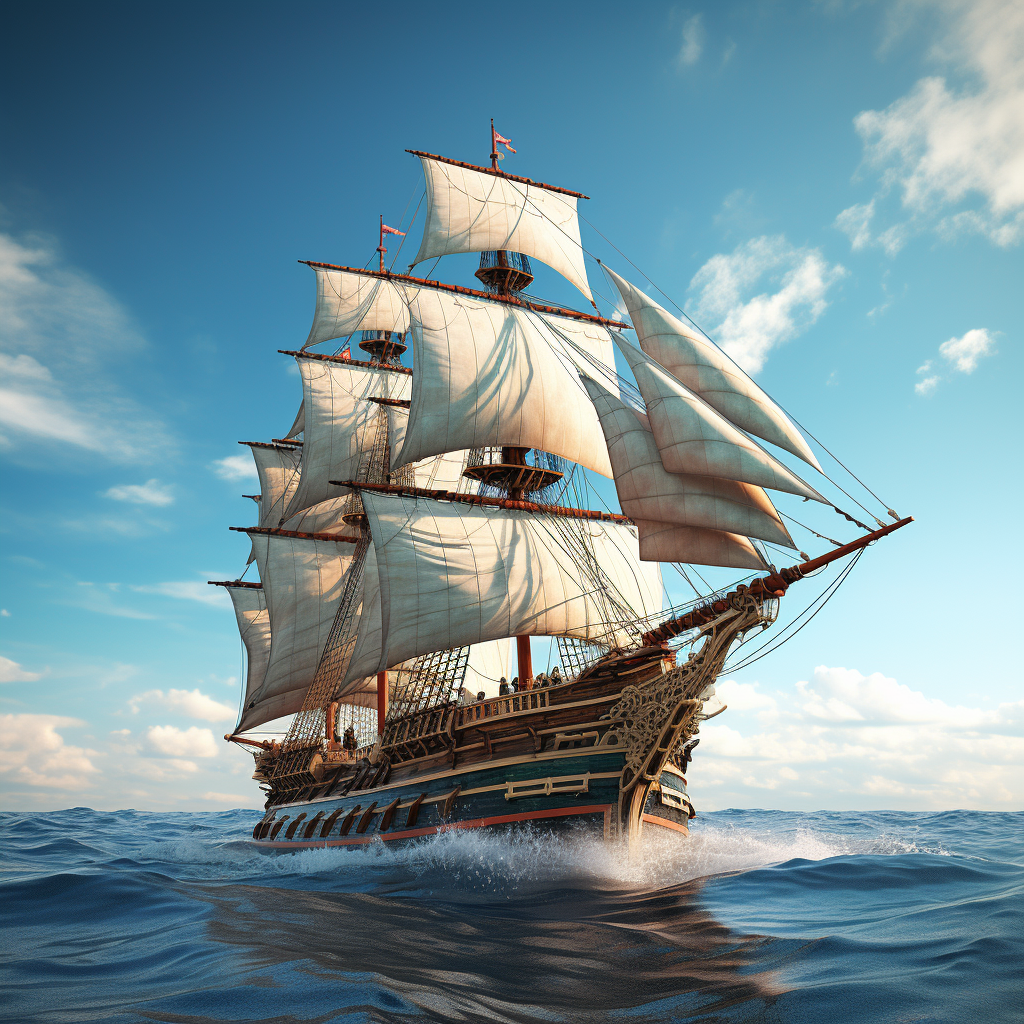
\includegraphics[width=\linewidth]{images/htwkleipzig_sailing_frigate_full_set_sails_calm_ocean_blue_sky__4060fe96-060b-4ddf-890a-349f3de73f6f.png}
	\caption{Sailing Frigate. Image generated by Andreas Both (2023).}
	\label{fig:my-figure-1}
	\Description{A woman and a girl in white dresses sit in an open car.}
\end{figure}

\begin{figure*}[t]
	\centering
	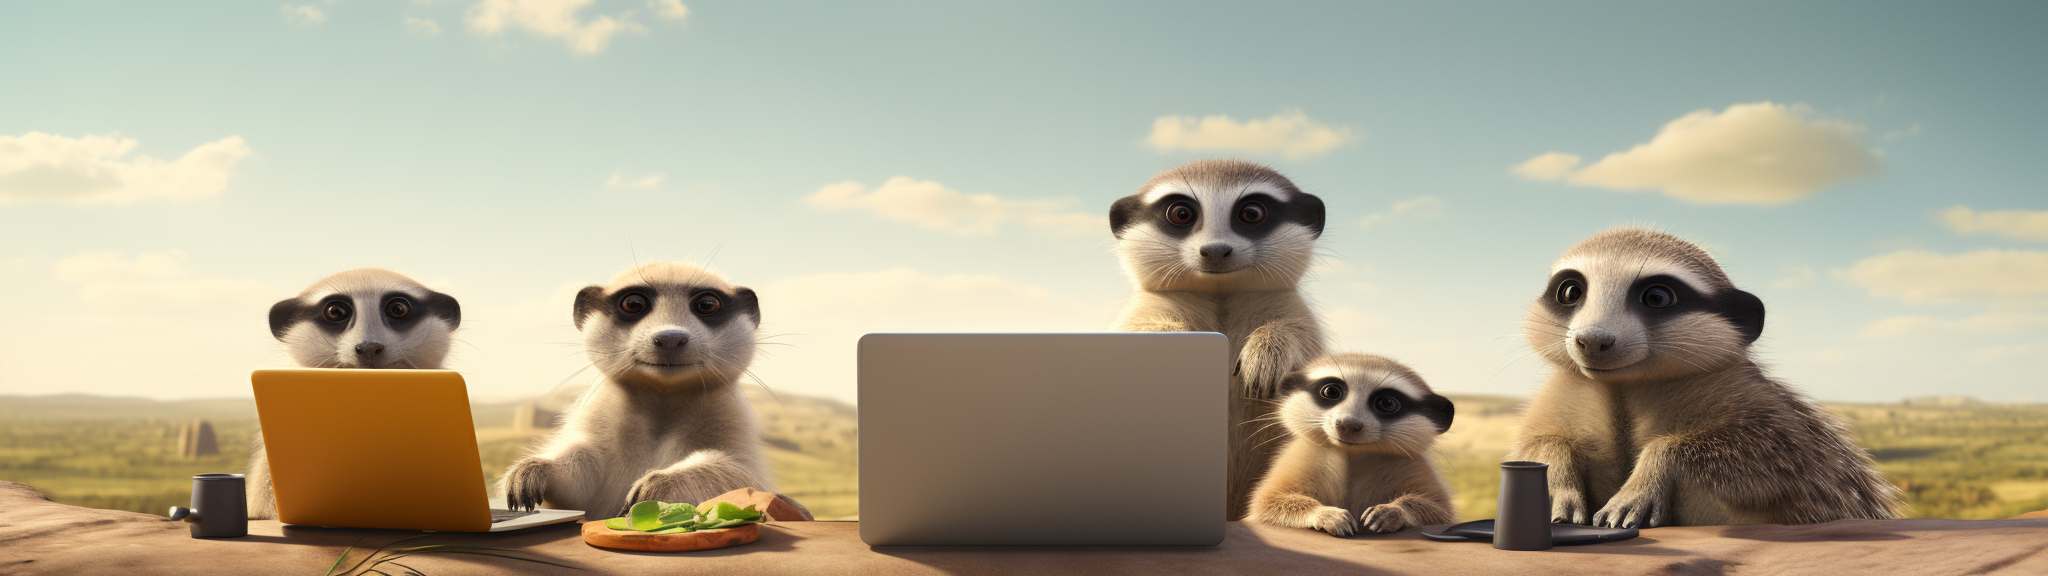
\includegraphics[width=\linewidth]{images/anbo_de_A_group_of_Meerkats_in_nature_working_on_laptops_super__fd9893f8-7134-4950-94ae-0a24ff6ae5f3.png}
	\caption{Meerkats in nature working on laptops. Image by Andreas Both (2023). (image with full page width)}
	\label{fig:my-figure-2}
	\Description{A woman and a girl in white dresses sit in an open car.}
\end{figure*}

Your figures (cf. Abb.~\ref{fig:my-figure-1} and \ref{fig:my-figure-2}) should contain a caption which describes the figure to
the reader.

Figure captions are placed {\itshape below} the figure.

Every figure should also have a figure description unless it is purely
decorative. These descriptions convey what’s in the image to someone
who cannot see it. They are also used by search engine crawlers for
indexing images, and when images cannot be loaded.

A figure description must be unformatted plain text less than 2000
characters long (including spaces).  {\bfseries Figure descriptions
		should not repeat the figure caption – their purpose is to capture
		important information that is not already provided in the caption or
		the main text of the paper.} For figures that convey important and
complex new information, a short text description may not be
adequate. More complex alternative descriptions can be placed in an
appendix and referenced in a short figure description. For example,
provide a data table capturing the information in a bar chart, or a
structured list representing a graph.  For additional information
regarding how best to write figure descriptions and why doing this is
so important, please see
\url{https://www.acm.org/publications/taps/describing-figures/}.

\subsection{The ``Teaser Figure''}

A ``teaser figure'' is an image, or set of images in one figure, that
are placed after all author and affiliation information, and before
the body of the article, spanning the page. If you wish to have such a
figure in your article, place the command immediately before the
\verb|\maketitle| command:
\begin{verbatim}
  \begin{teaserfigure}
    \includegraphics[width=\textwidth]{sampleteaser}
    \caption{figure caption}
    \Description{figure description}
  \end{teaserfigure}
\end{verbatim}

\subsection{Citations and Bibliographies}

Citations and references are numbered by default. A small number of
ACM publications have citations and references formatted in the
``author year'' style; for these exceptions, please include this
command in the {\bfseries preamble} (before the command
``\verb|\begin{document}|'') of your \LaTeX\ source:
\begin{verbatim}
  \citestyle{acmauthoryear}
\end{verbatim}


\section{Diskussion}

(Einordnung, Interpretation und Bewertung der Erkenntnisse -- (nachvollziehbare, begründbare) Meinungen sind erlaubt)

Some examples.  A paginated journal article \cite{Abril07}, an
enumerated journal article \cite{Cohen07}, a reference to an entire
issue \cite{JCohen96}, a monograph (whole book) \cite{Kosiur01}, a
monograph/whole book in a series (see 2a in spec. document)
\cite{Harel79}, a divisible-book such as an anthology or compilation
\cite{Editor00} followed by the same example, however we only output
the series if the volume number is given \cite{Editor00a} (so
Editor00a's series should NOT be present since it has no vol. no.),
a chapter in a divisible book \cite{Spector90}, a chapter in a
divisible book in a series \cite{Douglass98}, a multi-volume work as
book \cite{Knuth97}, a couple of articles in a proceedings (of a
conference, symposium, workshop for example) (paginated proceedings
article) \cite{Andler79, Hagerup1993}, a proceedings article with
all possible elements \cite{Smith10}, an example of an enumerated
proceedings article \cite{VanGundy07}, an informally published work
\cite{Harel78}, a couple of preprints \cite{Bornmann2019,
	AnzarootPBM14}, a doctoral dissertation \cite{Clarkson85}, a
master's thesis: \cite{anisi03}, an online document / world wide web
resource \cite{Thornburg01, Ablamowicz07, Poker06}, a video game
(Case 1) \cite{Obama08} and (Case 2) \cite{Novak03} and \cite{Lee05}
and (Case 3) a patent \cite{JoeScientist001}, work accepted for
publication \cite{rous08}, 'YYYYb'-test for prolific author
\cite{SaeediMEJ10} and \cite{SaeediJETC10}. Other cites might
contain 'duplicate' DOI and URLs (some SIAM articles)
\cite{Kirschmer:2010:AEI:1958016.1958018}. Boris / Barbara Beeton:
multi-volume works as books \cite{MR781536} and \cite{MR781537}. A
couple of citations with DOIs:
\cite{2004:ITE:1009386.1010128,Kirschmer:2010:AEI:1958016.1958018}. Online
citations: \cite{TUGInstmem, Thornburg01, CTANacmart}. Artifacts:
\cite{R} and \cite{UMassCitations}.


\section{Zusammenfassung und Ausblick}

 (Überblick über die gesamte Arbeit, Rückführung auf Aussagen aus Kapitel 1 durchführen, offene Punkte als neue Forschungsfragen definieren)

Papers may be written in languages other than English or include
titles, subtitles, keywords and abstracts in different languages (as a
rule, a paper in a language other than English should include an
English title and an English abstract).  Use \verb|language=...| for
every language used in the paper.  The last language indicated is the
main language of the paper.

The title, subtitle, keywords and abstract will be typeset in the main
language of the paper.  The commands \verb|\translatedXXX|, \verb|XXX|
begin title, subtitle and keywords, can be used to set these elements
in the other languages.  The environment \verb|translatedabstract| is
used to set the translation of the abstract.  These commands and
environment have a mandatory first argument: the language of the
second argument.  See \verb|sample-sigconf-i13n.tex| file for examples
of their usage.

%% The next two lines define the bibliography style to be used, and
%% the bibliography file.
\bibliographystyle{ACM-Reference-Format}
\bibliography{01-Requirements-Engineering}

%%
%% If your work has an appendix, this is the place to put it.
\appendix

\section{Anhang 1}

\subsection{Übungsaufgaben}

Lorem ipsum dolor sit amet, consectetur adipiscing elit. Morbi
malesuada, quam in pulvinar varius, metus nunc fermentum urna, id
sollicitudin purus odio sit amet enim. Aliquam ullamcorper eu ipsum
vel mollis. Curabitur quis dictum nisl. Phasellus vel semper risus, et
lacinia dolor. Integer ultricies commodo sem nec semper.

\subsection{Part Two}

Etiam commodo feugiat nisl pulvinar pellentesque. Etiam auctor sodales
ligula, non varius nibh pulvinar semper. Suspendisse nec lectus non
ipsum convallis congue hendrerit vitae sapien. Donec at laoreet
eros. Vivamus non purus placerat, scelerisque diam eu, cursus
ante. Etiam aliquam tortor auctor efficitur mattis.

\section{Anhang 2}

Nam id fermentum dui. Suspendisse sagittis tortor a nulla mollis, in
pulvinar ex pretium. Sed interdum orci quis metus euismod, et sagittis
enim maximus. Vestibulum gravida massa ut felis suscipit
congue. Quisque mattis elit a risus ultrices commodo venenatis eget
dui. Etiam sagittis eleifend elementum.

Nam interdum magna at lectus dignissim, ac dignissim lorem
rhoncus. Maecenas eu arcu ac neque placerat aliquam. Nunc pulvinar
massa et mattis lacinia.

\section{Anhang 3}

...

\end{document}
\endinput
%%
%% End of file `sample-acmtog.tex'.
